\section{Methodology}


In this section, we will propose the details of the baseline model that we will be comparing with including the network architecture, the data preprocessing steps, and the loss function. We will then show our proposed methods using self-supervised learning and how it helps to improve generalisation and performance of the model while having a limited number of data samples. We will also show the extension our data preprocessing steps which further improves the performance of our model.

\subsection{Baseline}
The baseline that we will be comparing with is Inf-Net (Lung Infection Segmentation Network) \cite{ref14} without using any semi-supervised learning algorithm. This is to show that the self-supervised learning method  improves the performance of the baseline supervised learning Inf-Net. 

\begin{figure*}
	\centering
	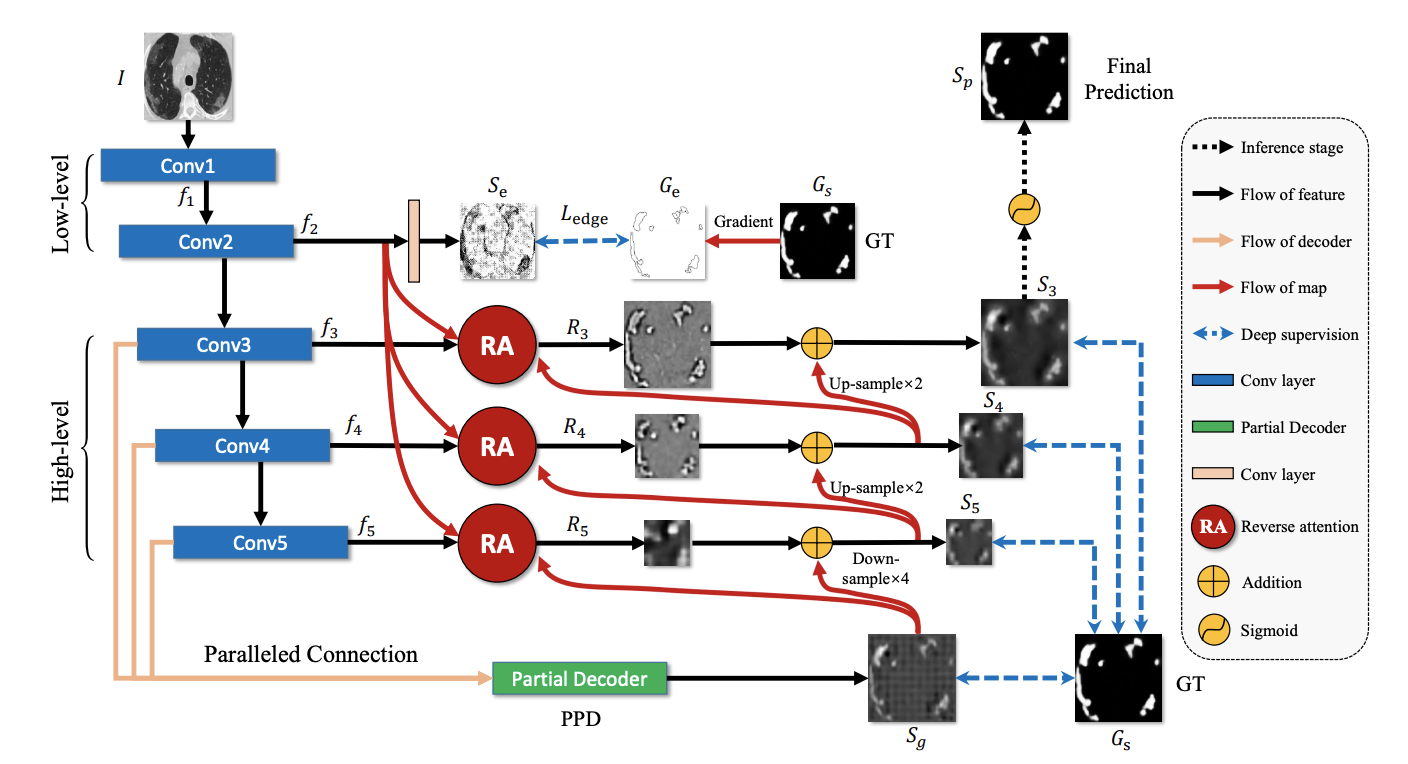
\includegraphics[width=\linewidth]{inf-net_architecture.png}
	\caption{The architecture of the inf-net model \cite{ref14}.}
	\label{fig:inf-net_arch}
\end{figure*}

The network architecture of Inf-Net is shown in \ref{fig:inf-net_arch}. The CT images are first passed through two convolution layers to extract the low-level features. The low-level features extracted will then be passed into three convolutional layers to obtain the high-level features. The low-level features are also passed into an edge attention module that helps to improve the representation of different boundaries for the segmentation. The high-level features from the three convolution layers are passed into a \textit{parallel partial decoder} (PPD) to aggregate the features and generate a map for the lung infections. The features generated by the PPD will then be calculated together with the high-level features generated by the previous three convolutional layers with a \textit{reverse attention } module. The equation of R is obtained by:
\begin{equation}
R_i = Concat(f_i, Downs(e_{att}))\odot A_i
\end{equation}

where $f_i$ refers one of the high-level features generated by one of the three convolutional layers, $e_{att}$ refers to the features before feeding into the edge attention module. The ${A_i}$ is obtained by:
\begin{equation}
A_i = \eta (\circleddash (\sigma (Upsample(S_{i+1}))))
\end{equation}

where S is the smaller predicted output from one level higher. $\sigma$ is the sigmoid operation to convert the output to range between [0, 1]. $\circleddash$ is the reverse operation by substracting the input from a matrix with all ones. $\eta$ is the expansion of the single tensor to 64 repeated tensors, reversing each candidate of the tensor.

There are several loss functions proposed for this baseline model. The first loss function is the loss edge, $L_{edge}$ which guides the model in representing better segmentation boundaries. The other loss function is the segmentation loss, ${L_{seg}}$. The segmentation loss combines both the loss of Intersection over Union (IoU) and the binary cross entropy loss. The segmentation loss equation is as follows:
\begin{equation}
L_{seg} = L_{IoU} + \lambda L_{BCE}
\end{equation}

The $\lambda$ is set to 1 for this experiment. The segmentation loss is adapted to all of the ${S_i}$ predicted output where ${S_i}$ are created from $f_i$ such that $i={3,4,5}$. The pseudo-code for the training of baseline model is relatively straightforward as can be seen in \ref{alg:baseline}.
\begin{algorithm}
	\caption{Pseudo code for Inf-Net}
	\label{alg:baseline}
\begin{algorithmic}
\STATE \textbf{Input:} Labeled data $D_{labeled}$
\FOR {each batch of $D_{labeled}$:}
\STATE $P_{labeled}$ = Preprocess $D_{labeled}$
\STATE Perform training of baseline Inf-Net, \textit{M}, on $P_{labeled}$
\STATE calculate test performance of \textit{M} on testing labeled data.
\STATE save model weights, \textit{w}.
\ENDFOR
\end{algorithmic}
\end{algorithm}

The total loss function for the baseline Inf-Net model is then:
\begin{equation}
L_{total} = L_{seg}(G_t, S_g) + L_{edge} + 	\sum_{i=3}^{5}L_{seg}(G_t, S_i)
\end{equation}

The summation of the loss functions are calculated from the output of the three convolutional layers. $G_t$ refers to the ground truth labels. $S_g$ is the output from the parallel partial decoder to match with the ground truth label.

\subsection{Self-supervised method}
In order to mitigate the problem of a limited number of data samples available and to aid in the generalisation of deep learning models, we  determine to use self-supervised learning to learn good representations of the CT scan of lung images. Self-supervised learning generates auxiliary tasks from the labeled data samples. For instance, when undergoing data augmentation with rotation, we could train the network to predict if the images have been rotated 0 degree, 90 degree, 180 degree to learn representations of the images. 

We will propose using a self-supervised method to improve the performance of deep neural networks to create pixel-level segmentation for CT scan for lung images of COVID-19 patients. We will integrate self-supervised inpainting to pre-train our network. As shown in \cite{ref25}, image inpainting is similarly related to image segmentation. By learning features from Image inpainting, the model can learn more features that are related to image segmentation. As creating mask can be a complex task for the network to learn to inpaint, the mask can either be too complex for the network to start learning or too simple to be able to learn good representations. We will be using a coach network\cite{ref25} that increases the complexity of the masking of the CT images throughout the training of the network. The mask created will initially be relatively simple, once the network is able to predict the inpainting of the CT images with good performance, the coach will increase the complexity of the masking to reduce the performance of the network, similar to how Generative Adversarial Network (GAN) \cite{ref20} works. The loss fuction for the coach network is:
\begin{equation}
L_{coach}(x) = 1 - L_{rec}(x\odot M)
\end{equation}

where $M = C(x)$ which is created by the coach network. A constraint is apply to this loss function because the coach network would just create a mask that masks all region because no context information would be present for the network to learn and a maximum loss will be achieved. The constraint is:
\begin{equation}
\hat{B}(x) = B(x) - SORT(B(x))^{k|B(x)} 
\end{equation}
\begin{equation}
M = C(x) = \sigma (\alpha \hat{B}(x))
\end{equation}

The backbone, B, of the coach network has a similar network architecture with the model that inpaints the CT images. SORT(B(x)) sorts the features in descending order over the activation map. k represents the $k^{th}$ elements in the sorted list and k helps to control the fraction of the image to be erased. The region that has scores lesser than the $k^{th}$ element will be erased from the images. If k is 0.75 then 0.75 fraction of the images will not be erased. The score is scaled into a range of [0, 1] using a sigmoid activation function. We keep $\alpha = 1$ while training the coach network.

\begin{algorithm}
	\caption{Pseudo code for self-supervised with Inf-Net}
	\label{alg:self-inf-net}
	\begin{algorithmic}
		\STATE \textbf{Input:} Labeled data $D_{labeled}$
		\FOR {each epoch}
			\FOR{each coach step}
			\STATE Generate Mask using coach network
			\STATE Use the generated mask to masks the CT images
			\STATE calculate the loss for coach network
			\STATE backpropagate and adjust the mask accordingly
			\ENDFOR
			\FOR {each network step}
			\STATE Preprocessed $D_{labeled}$ with data augmentation to create $P_{labeled}$
			\STATE Generate inpainted output using inf-net network with last layer replaced by an inpaint layer
			\STATE Calculate inpainting loss and back-propagate
			\ENDFOR
		\ENDFOR 
		

		\FOR {each batch of $D_{labeled}$:}
		\STATE $P_{labeled}$ = Preprocess $D_{labeled}$
		\STATE Perform training of baseline Inf-Net, \textit{M}, on $P_{labeled}$
		\STATE calculate test performance of \textit{M} on testing labeled data.
		\STATE save model weights, \textit{w}.
		\ENDFOR
	\end{algorithmic}
\end{algorithm}

We will also implement different data augmentation that includes random cropping, rotation, and random cutout \cite{ref7,ref15,ref16} to increase the number of available annotated data samples and labels as well as improve the model generalization as the data samples for CT images from COVID-19 can be limited.

Once the network is able to predict the pixel-level segmentation of the CT scan images, we will determine the severity score of the lung regions through several methods. The severity score of the lungs can be determined by using CT severity score (CT-SS) \cite{ref11}. The score uses lung opacification for extension of the infections in the lungs. CT-SS is an adaptation from the method previously used in patients after severe-acute respiratory syndrome (SARS) \cite{ref10} to describe ground-glass opacity, interstitial opacity, and air trapping. The lungs will be divided into 20 regions, the posterior apical segment of upper left lobe was divided into apical and posterior segmental regions, the anteromedial basal segment of lower left lobe will be divided into anterior and basal segmental regions. For each region, there contain a system attributing scores of 0, 1, 2, either parenchymal opacification involves 0%, less than 50%, or equal to or more than 50%. The CT-SS will calculate the sum of individual scored regions. The final value of CT-SS can range from 0 to 40.

Another method to determine the severity score is to use Dice similarity coefficient (DSC) \cite{ref12}  to evaluate the overlap ratio between the automatically segmented regions by the network and the reference region provided by radiologists. The equation is as follows:

\begin{equation}
DSC(R,S)=\frac{2|R\cap S|}{|R|+|S|}
\end{equation}

Where R refers to the reference region provided by the radiologists and S refers to the automatically segmented regions by the network. $|.|$
is the operator that is used to calculate the number of voxels in a given region.

We will compare our method against supervised and semi-supervised \cite{ref13,ref14} models trained on COVID-19 dataset. For comparing supervised learning, we will compare against the paper \cite{ref13}. We will train and follow using the same network structure but change from supervised learning to self-supervised learning and compare the performance between supervised and self-supervised.

When comparing with the semi-supervised model, we determine that our model is successful if our model is able to reach close to or better than the performance of the semi-supervised model as semi-supervised model is able to obtain a higher amount of data samples by looking at both unannotated and annotated data samples while self-supervised model only have access to the annotated labels. A self-supervised learning method will create its own training annotated labels without any manual human labelling and trained without any unlabeled data samples. We will compare our method’s performance against Inf-Net \cite{ref14} which uses semi-supervised learning by generating pseudo labels from randomly selected unlabeled CT images.

Our method will be novel compare to the other methods mentioned as our method will be integrating both the segmentation of the CT lung images as well as the calculation of the severity score through caluclation of the segmented infected lung areas.


